\section{Example of the Results}

An example of the results was made for luminaire MSTR~SLB~4x18W. Elumdata were taken from a software \uv{Building Design}. The luminous intensity curve is shown in the figure~\ref{fig:IDiag}. The grid distances were chosen $600$~mm to respect the luminaire dimensions. The luminaire dimensions were $595\times 595\times 80$~mm.

The target maintained illuminance was set to $510$~lx to make sure that the result overcome the minimum value $500$~lx. The maintenance factor $MF$ was set  to $0.75$ by author's choice. There is only little effect of this parameter on processing of the algorithm. So it does not matter on the value to much in fact. Whole settings are summarized in table~\ref{tab:trgVal}. All luminaires have the same orientation defined by a \uv{axis vector}. The vector is the normal vector of the $C0^\circ-C180^\circ$ plane. The facet's area on all walls, ceiling and floor was rectangular with length of a side $250$~mm.

The results of the calculations are shown in the figure~\ref{fig:resCS} and the figure~\ref{fig:resAS}. There is presented one of the outputs for the center and the axis symmetry.  Calculated outputs are presented in table~\ref{tab:resVal}. Both 3D graphs (\ref{fig:resCS:E}~and~\ref{fig:resAS:E}) represent the illuminance without $MF$ correction. Therefore most of the values of illuminance are higher than the output maintained average illuminace $\overline{E}_{m}$.

According to the fitness in table~\ref{tab:resVal}, the center symmetry solution is better. Its advantage is related especially to higher uniformity. However this solution uses two more luminaires in comparison to the solution with the axis symmetry. Higher fitness in the case of center symmetry is common but it does not occur under any circumstances. Because of the symmetry behavior, the axis symmetry solution is capable to add luminaires by 4 while center symmetry solution add luminaires by 2. The value of maintained illuminance $\overline{E}_{m}$ is closer to the target value in the case of axis symetry solution. Adding 4 more luminaires would make this value too high. The resulting fitness would be smaller even though the uniformity would be possibly better.

It seems that the fitness function still does not respect all designer's requirements. Even the higher fitness is in the case of center symmetry solution, the better solution would possible be the one with the axis symmetry. First of all the positions of luminaries are in prettier and more traditional form here. The uniformity is lower, but since it fulfills the standard's requirements, it does not matter. At last the count of luminaires is lower. That conclude to less investments to a lighting system and its costs.

\begin{figure}[htb]
  \centering
  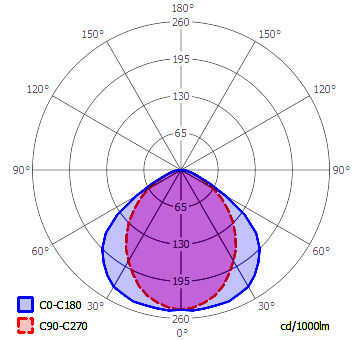
\includegraphics[width=0.7\columnwidth]{IDiag}
  \caption{Luminous intensity distribution curve of the luminaire sample}
  \label{fig:IDiag}
\end{figure}

\begin{table}[htb]
	\renewcommand{\arraystretch}{1.3}
	\caption{Target Values and Settings}
 	\label{tab:trgVal}
	\centering
  \begin{tabular}{| l | c |}
    \hline
    $\overline{E}_{m}$ (lx) & $510$ \\
    \hline
    $U_{0}$ (-) & $0.6$ \\
    \hline
		$MF$ & $0.75$ \\
    \hline
		Luminaire axis vector & $\left\langle 010\right\rangle$ \\
    \hline
		Grid ($N_x \times N_y$) & $16 \times 8$ \\
    \hline
		Grid distance from the walls (m) & $D_x=0.5, D_y=0.4$ \\
    \hline
  \end{tabular}
\end{table}

\begin{table}[htb]
	\renewcommand{\arraystretch}{1.3}
	\caption{Result Values}
 	\label{tab:resVal}
	\centering
  \begin{tabular}{| l | c | c |}
	  \hline
	  \textbf{Parameter} & \textbf{Central sym.} & \textbf{Axis sym.}\\
    \hline
    $\overline{E}_{m}$ (lx) & $526.9$ & $511.8$ \\
    \hline
    $U_{0}$ (-) & $0.81$ & $0.71$ \\
    \hline
		Luminaire count (-) & $18$ & $16$ \\
    \hline
		Fitness (-) & $1.616$ & $1.579$ \\
    \hline
  \end{tabular}
\end{table}

\begin{figure}[t]
        \centering
        \subfloat[3D graph of the illuminance \label{fig:resCS:E}]{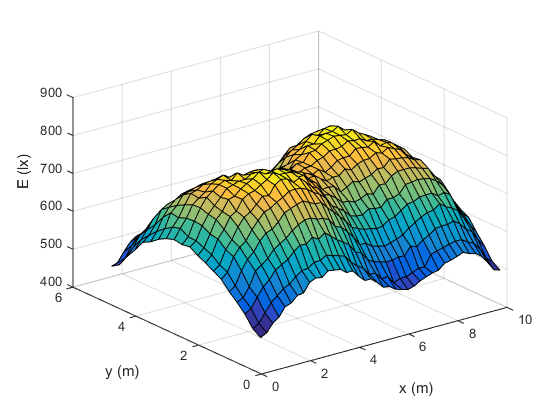
\includegraphics[width=\columnwidth]{../Vysledky/MSTR_SLB_4x18W_5G4_SR075_V010_S0_F1}}\\
        \subfloat[Luminaire positions \label{fig:resCS:P}]{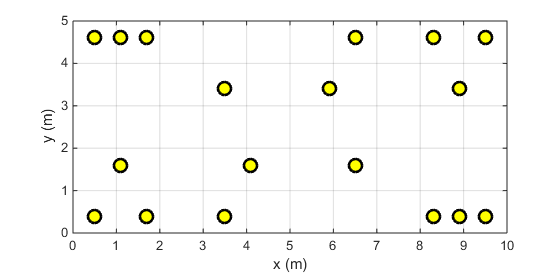
\includegraphics[width=\columnwidth]{../Vysledky/MSTR_SLB_4x18W_5G4_SR075_V010_S0_F2}}\\
        \subfloat[Best fitness during optimization \label{fig:resCS:F}]{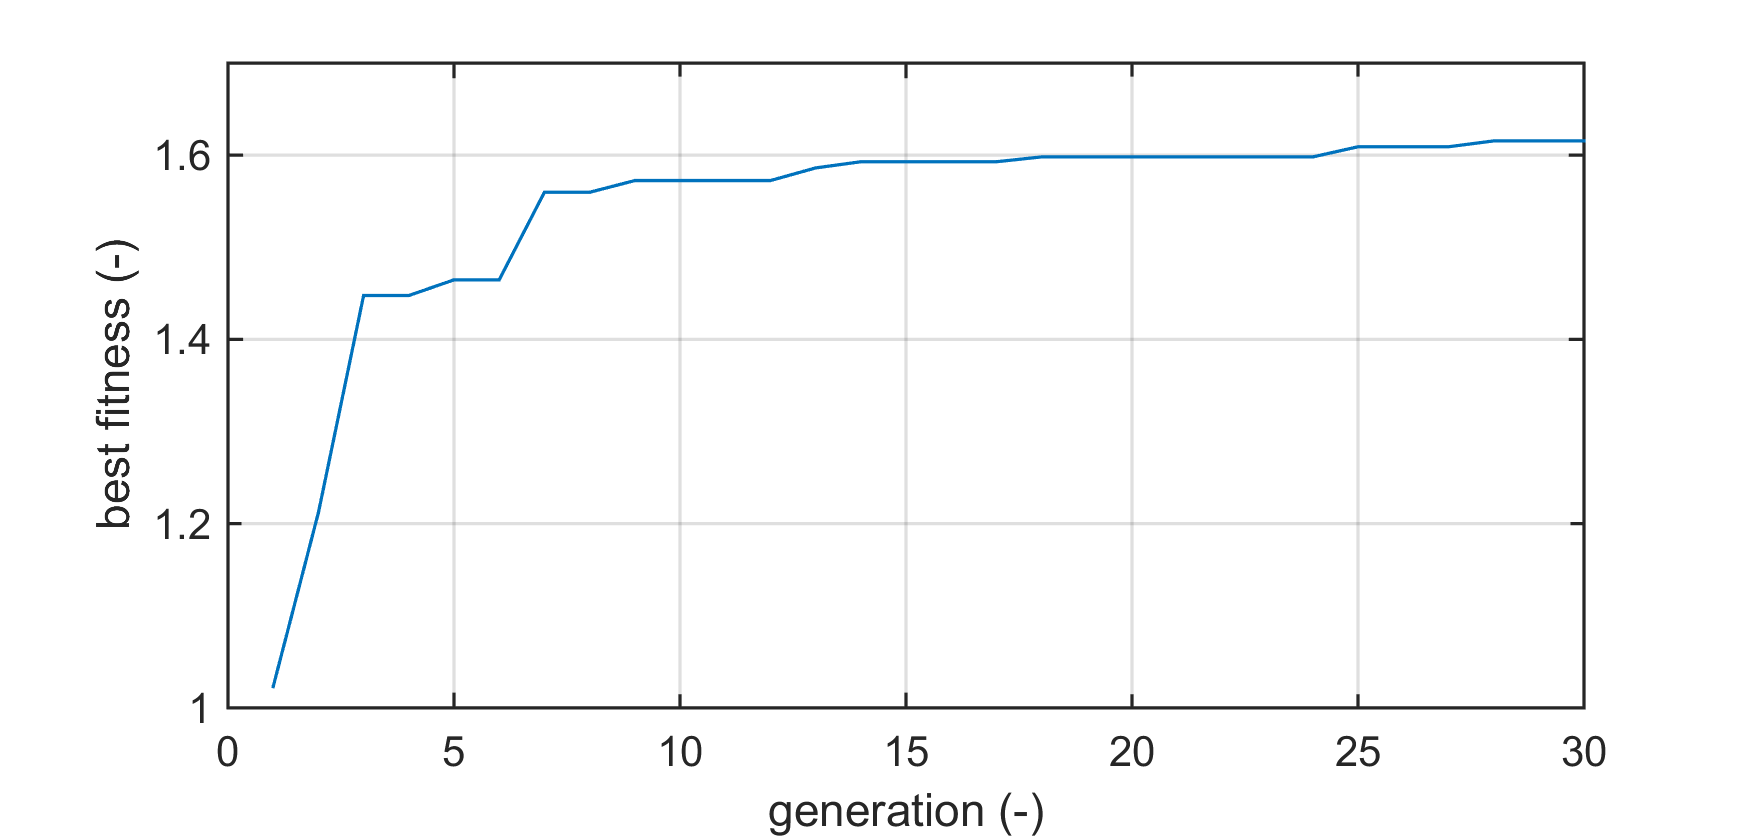
\includegraphics[width=\columnwidth]{../Vysledky/MSTR_SLB_4x18W_5G4_SR075_V010_S0_F3}}
        \caption{Example of result for lamp MSTR SLB 4x18W and central placement symmetry}
        \label{fig:resCS}
\end{figure}

\begin{figure}[t]
        \centering
        \subfloat[3D graph of the illuminance \label{fig:resAS:E}]{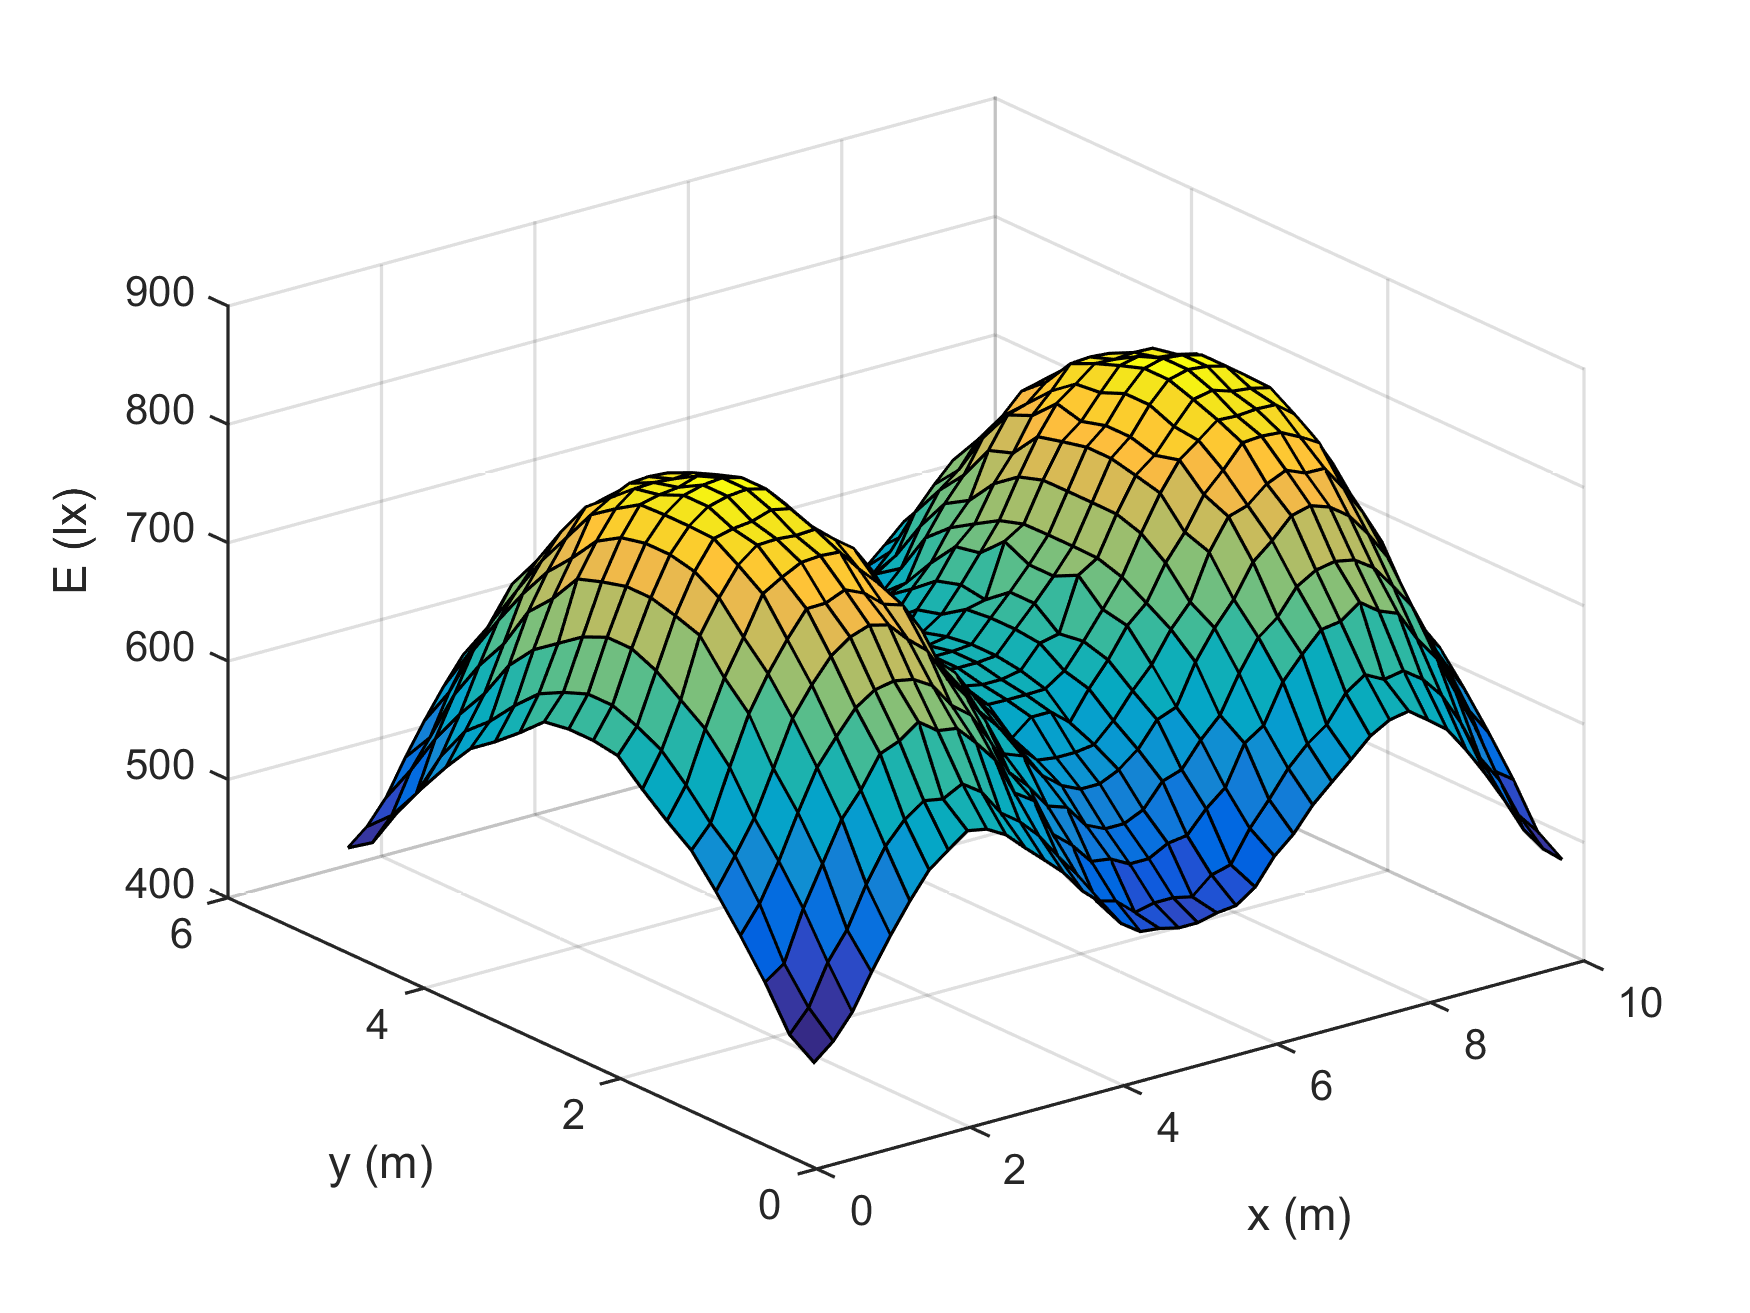
\includegraphics[width=\columnwidth]{../Vysledky/MSTR_SLB_4x18W_5G4_SR075_V010_S1_F1}}\\
        \subfloat[Luminaire positions \label{fig:resAS:P}]{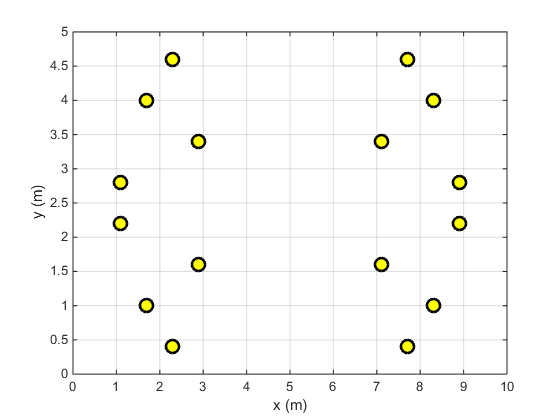
\includegraphics[width=\columnwidth]{../Vysledky/MSTR_SLB_4x18W_5G4_SR075_V010_S1_F2}}\\
        \subfloat[Best fitness during optimization \label{fig:resAS:F}]{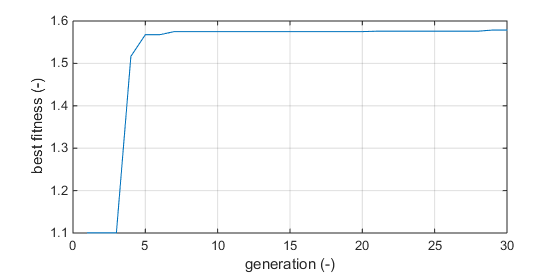
\includegraphics[width=\columnwidth]{../Vysledky/MSTR_SLB_4x18W_5G4_SR075_V010_S1_F3}}
        \caption{Example of result for lamp MSTR SLB 4x18W and axis placement symmetry}
				\label{fig:resAS}
\end{figure}